\begin{figure*}[t]
\centering
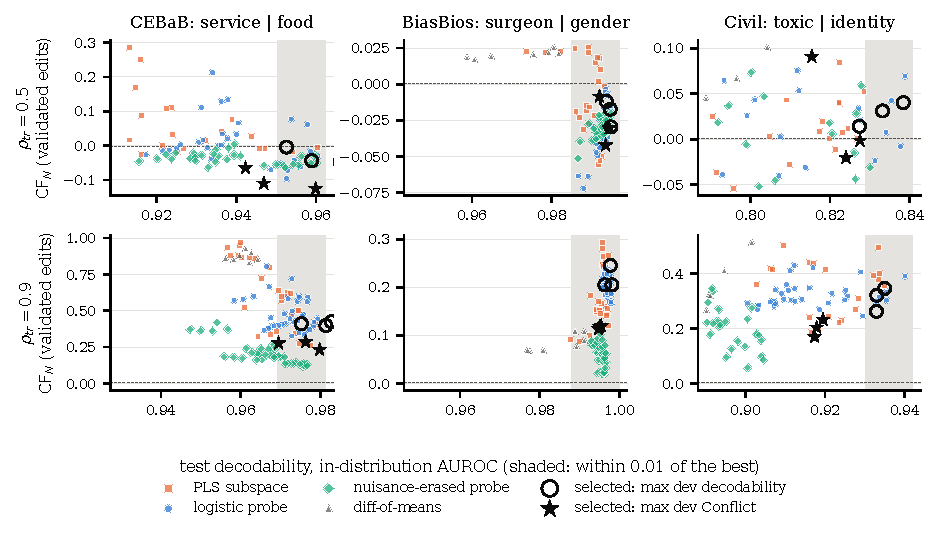
\includegraphics[width=\textwidth]{figs/fig_main_gemma9b.pdf}
\caption{As Figure~\ref{fig:main}, for Gemma-2-9B-it.}
\end{figure*}

\begin{table}[h]
\centering\small\setlength{\tabcolsep}{2pt}
\resizebox{\columnwidth}{!}{\begin{tabular}{@{}llccccc@{}}
\toprule
 & & best & \#near & $\cfn$ near-best & $\cfn$ equiv. & \conf{} \\
 & & \dec{} & (equiv.) & range & range & range \\
\midrule
\multicolumn{7}{@{}l}{\emph{$\rhot=0.7$}}\\
CEBaB & Q & .934 & 18 (0) & .15--.54 & -- & .70--.86 \\
 & G & .967 & 13 (0) & .05--.26 & -- & .86--.93 \\
BiasBios & Q & .995 & 62 (0) & .00--.13 & -- & .96--.99 \\
 & G & .995 & 61 (0) & $-$.01--.10 & -- & .96--.99 \\
Civil & Q & .859 & 5 (0) & .14--.17 & -- & .64--.71 \\
 & G & .869 & 9 (0) & .09--.19 & -- & .66--.69 \\
\bottomrule
\end{tabular}
}
\caption{As Table~\ref{tab:near}, at $\rhot=0.7$ (equivalence tests were run at $\rhot\in\{0.5,0.9\}$ only).}
\end{table}

\begin{table}[h]
\centering\small\setlength{\tabcolsep}{2pt}
\resizebox{\columnwidth}{!}{\begin{tabular}{@{}lllcccc@{}}
\toprule
data & model & $\rhot$ & $\cfn$ & $|\cfn|$ & \conf{} & $|$\leak{}$|$ \\
\midrule
BiasBios & G & 0.5 & $-$.32 [$-$.52, $-$.07] & +.10 [$-$.13, +.33] & +.90 [+.81, +.94] & $-$.24 [$-$.42, $-$.03] \\
BiasBios & G & 0.7 & +.41 [+.23, +.56] & +.40 [+.20, +.55] & +.69 [+.53, +.83] & +.59 [+.44, +.72] \\
BiasBios & G & 0.9 & +.39 [+.13, +.60] & +.39 [+.13, +.61] & +.52 [+.32, +.69] & +.40 [+.13, +.63] \\
BiasBios & Q & 0.5 & $-$.22 [$-$.45, +.05] & $-$.43 [$-$.62, $-$.22] & +.91 [+.84, +.95] & $-$.16 [$-$.38, +.10] \\
BiasBios & Q & 0.7 & $-$.01 [$-$.24, +.22] & $-$.01 [$-$.23, +.23] & +.75 [+.60, +.85] & +.35 [+.15, +.53] \\
BiasBios & Q & 0.9 & +.07 [$-$.24, +.34] & +.07 [$-$.22, +.35] & +.53 [+.32, +.70] & +.32 [+.04, +.53] \\
CEBaB & G & 0.5 & $-$.35 [$-$.57, $-$.03] & $-$.71 [$-$.83, $-$.51] & +.80 [+.64, +.89] & $-$.19 [$-$.46, +.10] \\
CEBaB & G & 0.7 & $-$.43 [$-$.67, $-$.15] & $-$.61 [$-$.77, $-$.36] & +.66 [+.45, +.81] & $-$.29 [$-$.55, +.02] \\
CEBaB & G & 0.9 & $-$.61 [$-$.75, $-$.42] & $-$.65 [$-$.78, $-$.46] & +.68 [+.52, +.78] & $-$.47 [$-$.63, $-$.27] \\
CEBaB & Q & 0.5 & $-$.23 [$-$.49, +.09] & $-$.65 [$-$.82, $-$.40] & +.74 [+.56, +.85] & $-$.08 [$-$.38, +.21] \\
CEBaB & Q & 0.7 & $-$.50 [$-$.67, $-$.23] & $-$.58 [$-$.74, $-$.36] & +.69 [+.51, +.79] & $-$.37 [$-$.57, $-$.11] \\
CEBaB & Q & 0.9 & $-$.43 [$-$.61, $-$.23] & $-$.46 [$-$.63, $-$.27] & +.35 [+.15, +.52] & +.20 [+.01, +.38] \\
Civil & G & 0.5 & +.05 [$-$.32, +.41] & $-$.51 [$-$.69, $-$.26] & +.67 [+.38, +.86] & +.43 [+.10, +.67] \\
Civil & G & 0.7 & $-$.20 [$-$.50, +.15] & $-$.30 [$-$.58, +.02] & +.24 [$-$.07, +.51] & +.53 [+.21, +.82] \\
Civil & G & 0.9 & +.03 [$-$.20, +.26] & $-$.02 [$-$.26, +.22] & $-$.25 [$-$.51, +.05] & +.66 [+.42, +.85] \\
Civil & Q & 0.5 & $-$.09 [$-$.40, +.26] & $-$.42 [$-$.63, $-$.13] & +.70 [+.43, +.84] & +.17 [$-$.22, +.50] \\
Civil & Q & 0.7 & $-$.01 [$-$.36, +.35] & $-$.08 [$-$.38, +.26] & +.24 [$-$.07, +.54] & +.53 [+.17, +.79] \\
Civil & Q & 0.9 & $-$.01 [$-$.29, +.29] & $-$.00 [$-$.30, +.33] & $-$.47 [$-$.69, $-$.20] & +.74 [+.49, +.91] \\
\bottomrule
\end{tabular}
}
\caption{Spearman correlation of test \dec{} with each facet across competitive standard extractors, with 95\% bootstrap CIs over extractors. Hyperparameter variants of one family are not independent, so CIs are descriptive.}
\end{table}

\begin{table}[h]
\centering\small\setlength{\tabcolsep}{2pt}
\resizebox{\columnwidth}{!}{\begin{tabular}{@{}lllcccc@{}}
\toprule
data & model & $\rhot$ & $\Delta$\dec{} [90\% CI] & equiv. & $\cfn$ probe & $\cfn$ erased \\
\midrule
BiasBios & G & 0.5 & $-$.000 [$-$.000, +.000] & yes & $-$.01 & $-$.03 \\
BiasBios & G & 0.9 & +.001 [$-$.001, +.002] & yes & .20 & .06 \\
BiasBios & Q & 0.5 & +.000 [$-$.000, +.000] & yes & $-$.00 & $-$.02 \\
BiasBios & Q & 0.9 & +.001 [+.000, +.002] & yes & .20 & .06 \\
CEBaB & G & 0.5 & +.000 [$-$.000, +.001] & yes & $-$.00 & $-$.01 \\
CEBaB & G & 0.9 & +.004 [$-$.003, +.012] & no & .63 & .14 \\
CEBaB & Q & 0.5 & $-$.003 [$-$.006, +.000] & yes & .13 & .02 \\
CEBaB & Q & 0.9 & +.009 [$-$.003, +.023] & no & .83 & .34 \\
Civil & G & 0.5 & +.008 [+.005, +.011] & no & .01 & $-$.01 \\
Civil & G & 0.9 & +.039 [+.031, +.049] & no & .26 & .18 \\
Civil & Q & 0.5 & +.011 [+.006, +.015] & no & .06 & .04 \\
Civil & Q & 0.9 & +.049 [+.036, +.062] & no & .40 & .28 \\
\bottomrule
\end{tabular}
}
\caption{Logistic probe vs.\ nuisance-erased probe, each family's layer and hyperparameter chosen on development \dec{} (training sample 0). Equiv.: 90\% CI of the \dec{} difference within $\pm0.01$.}
\end{table}

\paragraph{Readout ablation.} Reading the last non-special token instead of mean pooling (Qwen2.5-7B, Table~\ref{tab:pooling}) preserves the pattern: under correlated training, near-best extractors differ substantially in $\cfn$, decorrelated training largely removes it, and Conflict-based selection lowers $\cfn$. On Civil the last-token readout is less decodable and the selection costs considerably more accuracy.

\IfFileExists{tables/tab_pooling.tex}{\begin{table}[h]
\centering\small\setlength{\tabcolsep}{2pt}
\resizebox{\columnwidth}{!}{%
\begin{tabular}{@{}llccccc@{}}
\toprule
 & & \multicolumn{2}{c}{$\rhot=0.9$} & \multicolumn{2}{c}{$\rhot=0.5$} & selection, $\rhot=0.9$ \\
data & readout & best \dec{} & $\cfn$ near-best & best \dec{} & $\cfn$ near-best & $\cfn$: \dec{}$\to$\conf{} ($\Delta$\dec{}) \\
\midrule
CEBaB & mean & .966 & .46--.89 & .924 & .02--.28 & .69$\to$.54 ($-$.012) \\
CEBaB & last token & .968 & .51--.76 & .921 & .15--.27 & .56$\to$.49 ($-$.003) \\
BiasBios & mean & .998 & .08--.41 & .995 & $-$.04--.04 & .20$\to$.12 ($-$.001) \\
BiasBios & last token & .998 & .09--.66 & .994 & $-$.05--.01 & .27$\to$.09 ($-$.005) \\
Civil & mean & .932 & .24--.45 & .829 & .04--.08 & .43$\to$.33 ($-$.018) \\
Civil & last token & .904 & .67--.67 & .794 & .01--.05 & .67$\to$.09 ($-$.156) \\
\bottomrule
\end{tabular}}
\caption{Readout ablation (Qwen2.5-7B, standard extractors, accepted edits): mean pooling vs.\ the last non-special token.}
\label{tab:pooling}
\end{table}
}{}

\begin{table*}[t]
\centering\small
\resizebox{\textwidth}{!}{\begin{tabular}{@{}ll|cccc|ccc@{}}
\toprule
 & & \multicolumn{4}{c|}{standard extractors: $\cfn$ ($\Delta$\dec{})} & \multicolumn{3}{c}{+ erased probe: $\cfn$ ($\Delta$\dec{})} \\
 & & max \dec{} & max \conf{} & min $|$\leak{}$|$ & \dec{}$-|$\leak{}$|$ & max \conf{} & min $|$\leak{}$|$ & \dec{}$-|$\leak{}$|$ \\
\midrule
CEBaB & Q & .69 & .54 ($-$.012) & .50 ($-$.013) & .52 ($-$.008) & .34 ($-$.007) & .34 ($-$.007) & .33 ($-$.011) \\
 & G & .41 & .26 ($-$.005) & .27 ($-$.004) & .26 ($-$.005) & .11 ($-$.004) & .12 ($-$.004) & .14 ($-$.010) \\
BiasBios & Q & .20 & .12 ($-$.001) & .08 ($-$.004) & .10 ($-$.021) & .03 ($-$.002) & .03 ($-$.002) & .03 ($-$.002) \\
 & G & .22 & .12 ($-$.002) & .11 ($-$.006) & .07 ($-$.017) & .02 ($-$.002) & .02 ($-$.001) & .02 ($-$.001) \\
Civil & Q & .43 & .33 ($-$.018) & .31 ($-$.001) & .37 ($-$.041) & .15 ($-$.034) & .31 ($-$.001) & .17 ($-$.038) \\
 & G & .31 & .20 ($-$.015) & .30$^\dagger$ ($-$.006) & .22$^\dagger$ ($-$.020) & .11 ($-$.036) & .30$^\dagger$ ($-$.006) & .11 ($-$.034) \\
\bottomrule
\end{tabular}
}
\caption{All development-set selection criteria at $\rhot=0.9$ (as Table~\ref{tab:select}), for standard extractors and with the nuisance-erased probe.}
\end{table*}
